\documentclass{article}

% PACKAGES
\usepackage[english]{babel}
\usepackage[T1]{fontenc}
\usepackage[letterpaper,top=1.5cm,bottom=1.5cm,left=3cm,right=3cm,marginparwidth=1.75cm]{geometry}
\usepackage{minted}
\usepackage{amsmath}
\usepackage{hyperref}
\usepackage{titlesec}
\usepackage{tocloft}
\usepackage{graphicx}
\usepackage[utf8]{inputenc}
\usepackage{array}
\usepackage{multirow}

% SETUP
\title{Projekt 1 - całkowanie}
\author{Aleksander Dygon - 151856}
\date{}

% table of contents links
\hypersetup{
    colorlinks = true,
    linkcolor = black
}

% domain range command, usage: \ci{start}{end}
\newcommand{\ci}[2]{\langle #1, #2 \rangle}

% space command, usage: \spa
\newcommand{\spa}[0]{\vspace{32pt}}

% paragraph command, usage \p{text}
\newcommand{\p}[1]{\paragraph{#1}\mbox{}\\}

% dots in chapters in table of contents
\renewcommand{\cftsecleader}{\cftdotfill{\cftdotsep}}

% DOCUMENT BEGIN
\begin{document}


\maketitle

Niniejszy projekt zakłada opracowanie programu oraz dokumentacji do obliczania całek oznaczonych funkcji jednej zmiennej z wykorzystaniem trzech różnych metod: metodą prostokątów, metodą trapezów oraz metodą Monte Carlo. Program będzie interaktywnie przyjmował zakresy całkowania od użytkownika. Każda z metod będzie zaimplementowana jako odrębna funkcja, przyjmująca wskaźnik do funkcji podcałkowej.

\section*{Implementacja programu:}
Program będzie obliczał całki oznaczone funkcji jednej zmiennej przy użyciu trzech metod: metodą prostokątów, metodą trapezów oraz metodą Monte Carlo. Zakres całkowania będzie podawany przez użytkownika.

\subsection*{Metoda prostokątów:}
Całka jest obliczana jako suma pól prostokątów, gdzie długość boku prostokąta odpowiada długości podprzedziału, a wysokość jest równa wartości funkcji na początku, w środku lub na końcu danego podprzedziału.

\subsection*{Metoda trapezów:}
Całka jest obliczana jako suma pól trapezów, gdzie długość podstaw trapezu jest równa wartościom funkcji na obu końcach podprzedziału.

\subsection*{Metoda Monte Carlo:}
Metoda polega na losowym generowaniu punktów w badanym przedziale i obliczaniu stosunku punktów znajdujących się pod wykresem funkcji do całkowitej liczby punktów. Wartości funkcji w badanym przedziale są wykorzystywane do określenia zakresu losowania punktów.

\section*{Schematy blokowe podanych metod}

\begin{figure}[H]
    \centering
    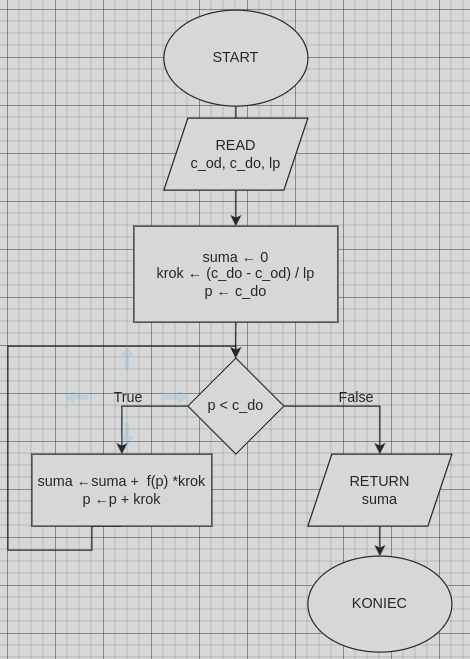
\includegraphics[width=\textwidth]{"../assets/prost.png"}
    \caption{Schemat blokowy całkowania metodą prostokątów}
    \label{fig:block_diagram_prost}
\end{figure}

\begin{figure}[H]
  \centering
  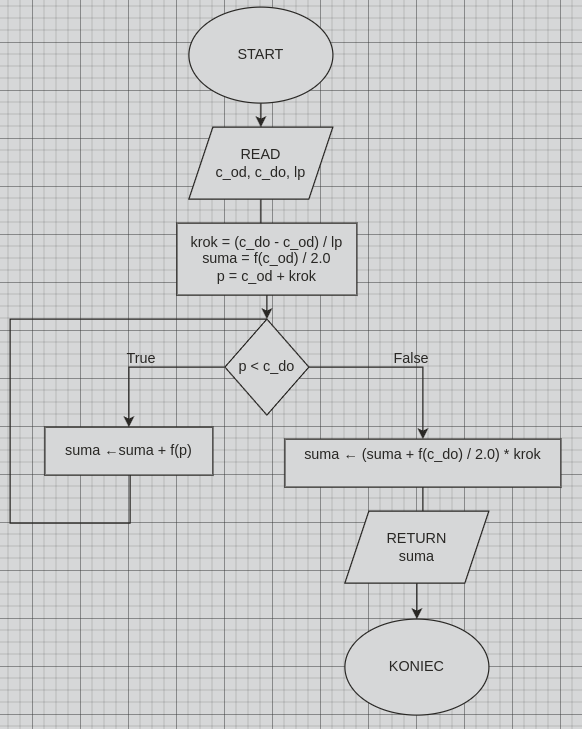
\includegraphics[width=\textwidth]{"../assets/trapez.png"}
  \caption{Schemat blokowy całkowania metodą trapezów}
  \label{fig:block_diagram_trapez}
\end{figure}


\begin{figure}[H]
  \centering
  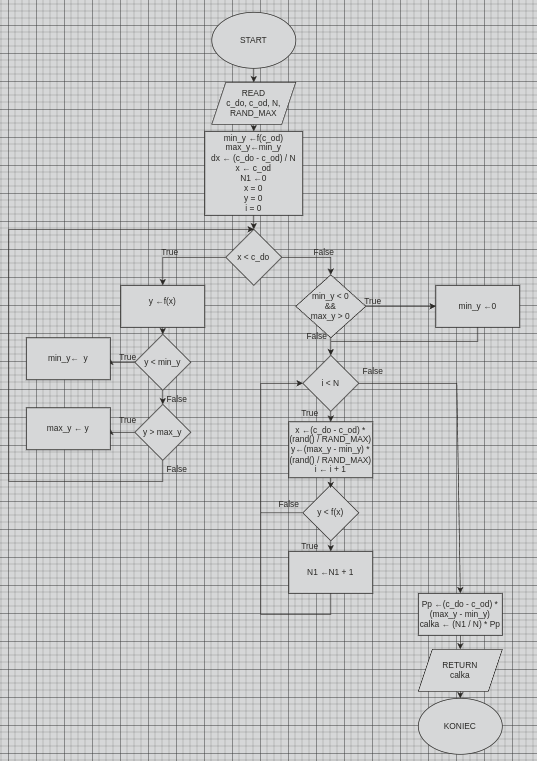
\includegraphics[width=\textwidth]{"../assets/mc.png"}
  \caption{Schemat blokowy całkowania metodą Monte Carlo}
  \label{fig:block_diagram_monte_carlo}
\end{figure}


\section*{Wykresy badanych funkcji w przedziale $[-10, 10]$}

\begin{figure}[H]
    \centering
    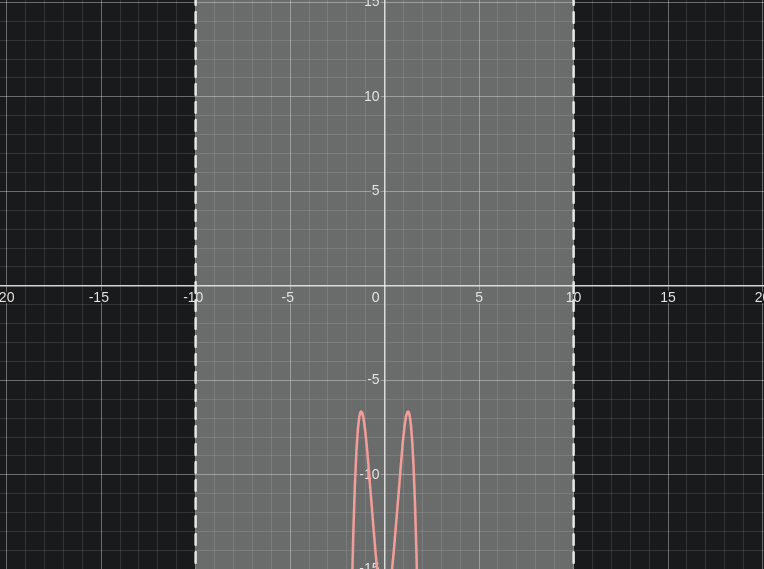
\includegraphics[width=\textwidth]{"../assets/f_1.png"}
    \caption{$f(x) = -4.4x^3 + 13.5x^2 - 17 $}
    \label{fig:f_1}
\end{figure}
  
\begin{figure}[H]
    \centering
    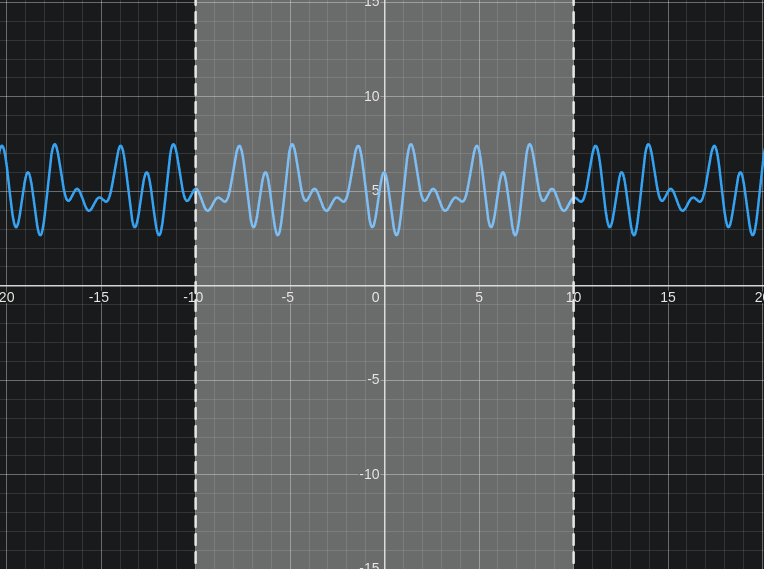
\includegraphics[width=\textwidth]{"../assets/f_2.png"}
    \caption{$f(x) = 2sin(3x) * sin(x-3) + cos(5x)$}
    \label{fig:f_2}
\end{figure}
\begin{figure}[H]
    \centering
    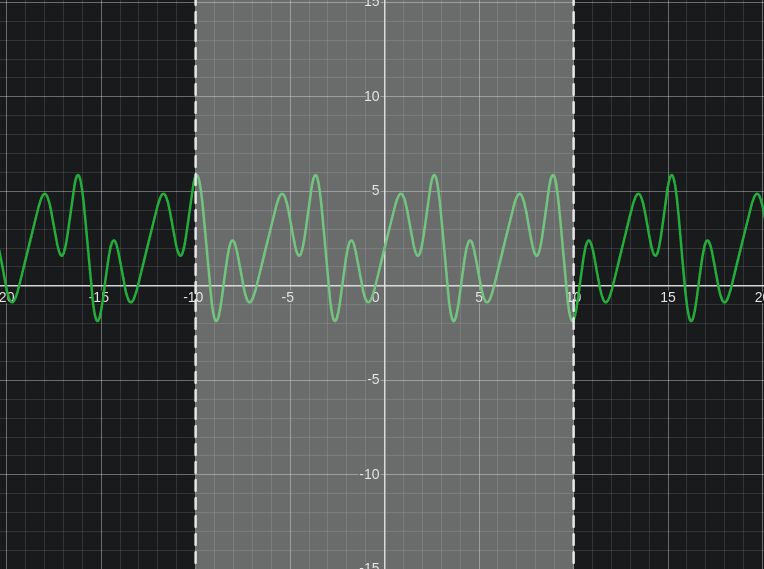
\includegraphics[width=\textwidth]{"../assets/f_3.png"}
    \caption{$f(x) = 4cos(x) * sin(2x) - sin(4x) + 2$}
    \label{fig:f_3}
\end{figure}
\begin{figure}[H]
    \centering
    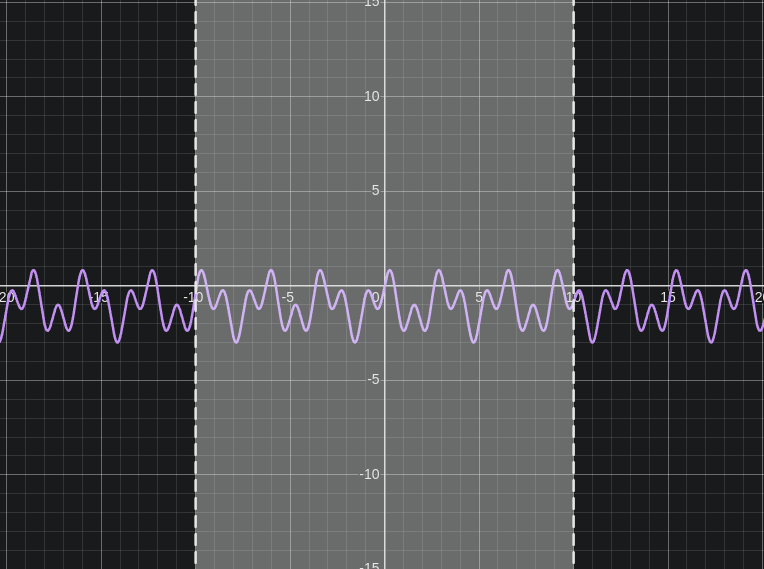
\includegraphics[width=\textwidth]{"../assets/f_4.png"}
    \caption{$f(x) = cos(2x) + sin(5x) - 1$}
    \label{fig:f_4}
\end{figure}

\clearpage

\section*{Rozwiazania analityczne}

${\int_{-10}^{10} -4.4x^3 + 13.5x^2 - 17 dx  = 8660}$ \newline \newline
${\int_{-10}^{10} 2sin(3x) * sin(x-3) + cos(5x) dx  \approx -0.63993}$ \newline \newline
${\int_{-10}^{10} 4cos(x) * sin(2x) - sin(4x) + 2 dx  = 40}$ \newline \newline
${\int_{-10}^{10} cos(2x) + sin(5x) - 1 dx  \approx -19.087}$

\section*{Wyniki}

\begin{table}[H]
    \begin{tabular}{|l|l|l|l|l|}
    \hline
                       & F1             & F2        & F3        & F4         \\ \hline
    Metoda Prostokatów & -167342.053924 & 99.366329 & 40.101579 & -19.080274 \\ \hline
    Metoda Trapezów    & -167342.053924 & 99.360089 & 40.000000 & -19.087271 \\ \hline
    Metoda Monte Carlo & 657538.214946  & 45.382964 & 43.806935 & 2.178229   \\ \hline
    Wynik Analityczny  & 8660           & -0.63993  & 40        & -19.087    \\ \hline
\end{tabular}
\end{table}


\section*{Podsumowanie}

W niniejszym projekcie zaimplementowano trzy różne metody numerycznego całkowania funkcji jednej zmiennej: metodę prostokątów, metodę trapezów oraz metodę Monte Carlo. Każda z tych metod została zaimplementowana jako oddzielna funkcja przyjmująca wskaźnik do funkcji podcałkowej oraz zakres całkowania. Program pozwala na interaktywne podawanie zakresu całkowania przez użytkownika.

\subsection*{Wnioski}

Na podstawie wyników obliczeń można wyciągnąć następujące wnioski:

\begin{itemize}
    \item \textbf{Metoda Prostokątów} wykazała znaczące różnice w porównaniu do wyników analitycznych, szczególnie dla funkcji \(f_1\). Wyniki tej metody są obarczone dużymi błędami, co może wynikać z wyboru podprzedziałów oraz charakterystyki funkcji.
    
    \item \textbf{Metoda Trapezów} dała wyniki znacznie bardziej zbliżone do wyników analitycznych niż metoda prostokątów, szczególnie dla funkcji \(f_3\) i \(f_4\). Metoda ta jest generalnie bardziej precyzyjna i stabilna, ponieważ lepiej aproksymuje obszar pod wykresem funkcji.
    
    \item \textbf{Metoda Monte Carlo} wykazała dużą zmienność wyników i w niektórych przypadkach dała wyniki znacznie odbiegające od wyników analitycznych, np. dla funkcji \(f_1\) i \(f_4\). Metoda ta jest silnie zależna od liczby losowo generowanych punktów oraz rozkładu tych punktów w przestrzeni.
    
    \item \textbf{Porównanie z wynikami analitycznymi} pokazuje, że metoda trapezów generalnie zapewnia najlepszą dokładność wśród testowanych metod, chociaż metoda Monte Carlo może być użyteczna dla funkcji, dla których inne metody zawodzą, szczególnie gdy analiza funkcji jest skomplikowana.
    
    \item \textbf{Zastosowania praktyczne} każdej z metod zależą od specyfiki problemu. Metody prostokątów i trapezów są prostsze w implementacji i często dają satysfakcjonujące wyniki dla funkcji o gładkich wykresach. Metoda Monte Carlo jest bardziej uniwersalna, ale jej dokładność zależy od liczby losowych próbek.
\end{itemize}

\end{document}